\documentclass[12pt, a4paper]{article}

% --- Pakiety ---
\usepackage[utf8]{inputenc}
\usepackage[T1]{fontenc}
\usepackage[polish]{babel}
\usepackage{geometry}
\usepackage{amsmath}
\usepackage{amssymb}
\usepackage{graphicx}
\usepackage{booktabs}
\usepackage{siunitx}
\usepackage{caption}
\usepackage{subcaption}
\usepackage{float}
\usepackage{hyperref}
\usepackage{xcolor}
\usepackage{array}
\usepackage{multirow}
\usepackage{fancyhdr}

% --- Marginesy ---
\geometry{
    top=2.5cm,
    bottom=2.5cm,
    left=2.5cm,
    right=2.5cm
}

% --- Stopka ---
\pagestyle{fancy}
\fancyhf{}
\renewcommand{\headrulewidth}{0pt}
\renewcommand{\footrulewidth}{0.4pt}
\fancyfoot[R]{
\includegraphics[height=0.8cm]{lumon.pdf}}

% --- Konfiguracja siunitx ---
\sisetup{
    output-decimal-marker = {,},
    separate-uncertainty = true
}

% --- Dane raportu ---
\newcommand{\tytul}{Wyznaczanie pojemności kondensatora metodą rozładowania}
\newcommand{\codeword}{St.~Pierre}
\newcommand{\nrCwiczenia}{E11}
\newcommand{\autor}{Karol Peszek}
\newcommand{\nrGrupy}{Grupa B}
\newcommand{\dataWykonania}{6 maja 2026}

% --- Tytuł dokumentu ---
\title{
    \large I Pracownia Fizyczna \\[0.5em]
    \textbf{Ćwiczenie \nrCwiczenia} \\[0.3em]
    \LARGE \tytul\space''\codeword''
}
\author{
    \autor\\
     Grupa \nrGrupy}
\date{
    Data wykonania pomiarów: \dataWykonania\\
}

% =============================================
\begin{document}
% =============================================

\maketitle
\thispagestyle{empty}
\newpage

% -------------------------------------------
\section{Cel ćwiczenia}
% -------------------------------------------

Celem ćwiczenia jest wyznaczenie pojemności kondensatora i~ładunku zgromadzonego
na jego okładkach metodą rozładowania w~obwodzie RC, a~także sprawdzenie wzorów
na pojemność zastępczą baterii kondensatorów połączonych równolegle oraz szeregowo.

% -------------------------------------------
\section{Wstęp teoretyczny}
% -------------------------------------------

\subsection{Pojemność kondensatora}

Kondensatorem nazywamy układ dwóch przewodników (zwanych okładkami) rozdzielonych
dielektrykiem. Jeżeli na okładkach kondensatora zgromadzony jest ładunek~$q$, to
między okładkami panuje różnica potencjałów (napięcie)~$U$, przy czym iloraz $q/U$
pozostaje stały. Wielkość tę nazywamy \emph{pojemnością kondensatora}:
\begin{equation}
    C = \frac{q}{U}.
    \label{eq:pojemnosc}
\end{equation}
Pojemność zależy od rozmiarów geometrycznych kondensatora oraz od rodzaju
dielektryka wypełniającego przestrzeń między okładkami. Jednostką pojemności
w~układzie SI jest farad ($1\,\mathrm{F} = 1\,\mathrm{C/V}$). W~praktyce stosowane
są jednostki podwielokrotne: milifarad, mikrofarad, nanofarad i~pikofarad
($10^{-3}\,\mathrm{F}$, $10^{-6}\,\mathrm{F}$, $10^{-9}\,\mathrm{F}$
i~$10^{-12}\,\mathrm{F}$).

\subsection{Rozładowanie kondensatora w obwodzie RC}

Szeregowy obwód RC składa się ze źródła napięcia~$U_0$, kondensatora~$C$,
opornika~$R$ oraz przełącznika~$P$ (rys.~\ref{fig:circuit}). Po naładowaniu
kondensatora do napięcia~$U_0$ i~przestawieniu przełącznika w~położenie
rozładowania, na okładkach kondensatora zgromadzony jest ładunek
\begin{equation}
    q = CU_0.
    \label{eq:ladunek}
\end{equation}
Gdy z~okładek odprowadzony zostaje ładunek $dq$, napięcie między okładkami maleje
o~$dU$, skąd:
\begin{equation}
    dq = C\,dU.
    \label{eq:dq}
\end{equation}
Przez opornik~$R$ płynie prąd~$I$ spełniający warunek:
\begin{equation}
    -dq = I\,dt,
    \label{eq:prad}
\end{equation}
a~ponieważ w~obwodzie mamy jedynie opór omowy:
\begin{equation}
    dU = R\,dI.
    \label{eq:ohm}
\end{equation}
Podstawiając równania (\ref{eq:prad}) i~(\ref{eq:ohm}) do równania (\ref{eq:dq})
i~przekształcając, otrzymujemy:
\begin{equation}
    \frac{dI}{I} = -\frac{1}{RC}\,dt.
    \label{eq:rozniczk}
\end{equation}
Po scałkowaniu:
\begin{equation}
    \ln\frac{I}{I_0} = -\frac{1}{RC}\,t,
    \label{eq:log}
\end{equation}
co można zapisać w~postaci równoważnej:
\begin{equation}
    I = I_0\,e^{-t/\tau},
    \label{eq:eksponenta}
\end{equation}
gdzie $\tau = RC$ jest \emph{stałą czasową obwodu}, a~$I_0 = U_0/R$ jest prądem
płynącym w~obwodzie w~chwili $t = 0$. Natężenie prądu rozładowania maleje więc
wykładniczo z~czasem z~szybkością określoną przez stałą~$\tau$.

Całkując równanie (\ref{eq:prad}) po czasie w~granicach $(0, \infty)$ oraz po
ładunku w~granicach $(q, 0)$, otrzymujemy zależność wiążącą ładunek
zgromadzony na kondensatorze ze stałą czasową i~wartością prądu początkowego:
\begin{equation}
    q = \tau I_0.
    \label{eq:ladunek_tau}
\end{equation}

\begin{figure}[H]
    \centering
    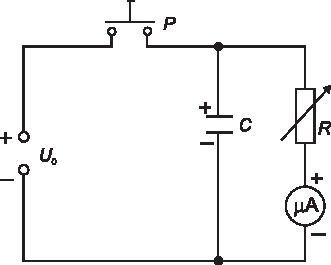
\includegraphics[width=0.5\textwidth]{circuit_schema.pdf}
    \caption{Schemat układu do wyznaczania pojemności kondensatora metodą
             rozładowania: $U_0$ --- źródło napięcia, $P$ --- przełącznik,
             $C$ --- kondensator, $R$ --- opornica dekadowa,
             $\mu\mathrm{A}$ --- mikroamperomierz. Źródło:~\cite{skrypt}.}\label{fig:circuit}
\end{figure}

\subsection{Łączenie kondensatorów}

Rozważamy połączenie równoległe i~szeregowe kondensatorów (rys.~\ref{fig:polaczenia}).

\paragraph{Połączenie równoległe.}
Przy połączeniu równoległym $n$~kondensatorów ta sama różnica potencjałów~$U_0$
jest przyłożona do każdego z~nich. Ładunek zgromadzony na $i$-tym kondensatorze
wynosi $q_i = C_i U_0$, a~całkowity ładunek baterii jest sumą ładunków na
poszczególnych kondensatorach. Pojemność zastępcza układu kondensatorów
połączonych równolegle jest sumą ich pojemności:
\begin{equation}
    C_r = \sum_{i=1}^{n} C_i.
    \label{eq:rownoleg}
\end{equation}

\pagebreak
\paragraph{Połączenie szeregowe.}
Przy połączeniu szeregowym $k$~kondensatorów przyłożona różnica potencjałów~$U_0$
jest równa sumie spadków napięć na poszczególnych kondensatorach
($U_0 = \sum_{j=1}^{k} U_j$). Zgodnie z~zasadą zachowania ładunku na wszystkich
kondensatorach gromadzą się jednakowe ładunki~$q$, a~napięcie na $j$-tym
kondensatorze wynosi $U_j = q/C_j$. Stąd odwrotność pojemności zastępczej
układu kondensatorów połączonych szeregowo jest sumą odwrotności pojemności
poszczególnych kondensatorów:
\begin{equation}
    \frac{1}{C_s} = \sum_{j=1}^{k} \frac{1}{C_j}.
    \label{eq:szereg}
\end{equation}

\begin{figure}[H]
    \centering
    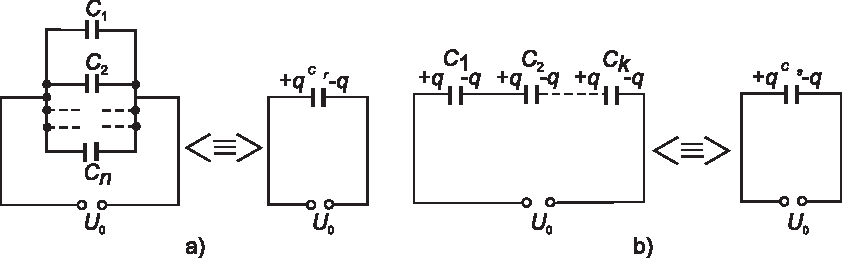
\includegraphics[width=0.85\textwidth]{capacitor_parallel_series.pdf}
    \caption{Łączenie kondensatorów: a.~równoległe --- pojemność zastępcza
             $C_r = \sum C_i$, b.~szeregowe --- pojemność zastępcza
             dana wzorem $1/C_s = \sum_j 1/C_j$. Źródło:~\cite{skrypt}.}\label{fig:polaczenia}
\end{figure}



% -------------------------------------------
\section{Opis układu pomiarowego}
% -------------------------------------------
\begin{figure}[H]
    \centering
    
\includegraphics[width=\textwidth]{schema.jpg}
    \caption{Fotografia układu pomiarowego.}\label{fig:schema}
\end{figure}

\subsection{Dostępne przyrządy i materiały}
Do przeprowadzenia pomiarów wykorzystano następujące przyrządy i materiały:
\begin{itemize}
    \item źródło napięcia stałego (zasilacz laboratoryjny) o~regulowanym potencjale 6V,
    \item opornica dekadowa o~zakresie oporów od 1~$\Omega$ do 100~k$\Omega$ i dokładności 50~$\Omega$,
    \item zestaw kondensatorów o~różnych, nieznanych pojemnościach,
    \item mikroamperomierz o~zakresie pomiarowym do 100~$\mu$A i dokładności 1.5~$\mu$A,
    \item przełącznik do zmiany trybu pracy układu (ładowanie/rozładowanie),
    \item przewody połączeniowe.
\end{itemize}

\subsection{Przygotowanie układu pomiarowego}

\begin{enumerate}
    \item Połączyć elementy układu zgodnie ze schematem przedstawionym na
          rysunku~\ref{fig:circuit}, upewniając się, że wszystkie połączenia są
          solidne i~bezpieczne.
    \item Ustawić opornicę dekadową na najwyższy opór (100~k$\Omega$) i~sprawdzić,
          czy mikroamperomierz wskazuje zero prądu.
    \item Przyłączyć układ do zasilacza i~ustawić napięcie na 6~V.
\end{enumerate}

% -------------------------------------------
\section{Procedura pomiarowa}
% -------------------------------------------

\begin{enumerate}
    \item Wcisnąć przełącznik w~położenie ładowania, a~następnie regulując
          opornicę dekadową ustawić prąd ładowania na~80~$\mu$A\@; zapisać tę
          wartość jako $I_0$ w~tabeli pomiarowej oraz zanotować wartość oporu~$R$.
    \item Włączyć stoper.
    \item Jednocześnie zwolnić przełącznik i~nacisnąć przycisk okrążenia stopera,
          aby rozpocząć pomiar czasu rozładowania kondensatora.
    \item Co 10~$\mu$A naciskać przycisk okrążenia stopera, aż prąd rozładowania
          spadnie do około 10~$\mu$A.
    \item Zanotować wartości prądu $I_n$ i~odpowiadające im czasy rozładowania
          w~tabeli pomiarowej.
    \item Powtórzyć pomiar pięciokrotnie dla danego układu.
    \item Powtórzyć serie pomiarowe dla każdego z~kondensatorów osobno, a~następnie
          dla ich połączenia równoległego i~szeregowego.
    \item Rozłączyć układ i~odłączyć zasilacz po zakończeniu pomiarów.
\end{enumerate}



% -------------------------------------------
\section{Wyniki pomiarów}
% -------------------------------------------

Opór dekadowy zastosowany we wszystkich pomiarach wynosił
$R = \SI{77700 \pm 50}{\ohm}$.
Niepewność wskazania mikroamperomierza wynosi $u_I = \SI{1,5}{\micro\ampere}$,
a~niepewność stopera $u_t = \SI{0,4}{\second}$, co jest typowym czasem reakcji osoby obsługującej stoper.
Czasy podane w~tabelach są wartościami bezwzględnymi odczytanymi ze stopera.
Na wykresach i~w~obliczeniach czasy zostały przesunięte tak, że $t = 0$
odpowiada odczytowi stopera w~chwili $I = \SI{80}{\micro\ampere}$ --- przesunięcie
wyznaczono \emph{osobno dla każdej serii} jako czas zanotowany przy $I_0 = \SI{80}{\micro\ampere}$
w~tej serii.

Nominalne napięcie zasilacza $U_0 = \SI{6}{\volt}$ dawałoby teoretycznie
$I_0 = U_0/R \approx \SI{77,2}{\micro\ampere}$, podczas gdy zmierzono
$I_0 = \SI{80}{\micro\ampere}$ (różnica $\approx 3{,}5\%$). Rozbieżność
wynika najprawdopodobniej z~rzeczywistego napięcia zasilacza odbiegającego
od wartości nominalnej --- typowa tolerancja zasilaczy laboratoryjnych wynosi
$1$--$2\%$. Opory wewnętrzne mikroamperomierza i~przewodów są pomijalnie małe
w~porównaniu z~$R = \SI{77700}{\ohm}$. Ponieważ kluczowa jest \emph{zmierzona}
wartość $I_0 = \SI{80}{\micro\ampere}$ wstawiana do wzoru $q = \tau I_0$,
rozbieżność ta nie wpływa na wyniki obliczeń.

\subsection{Kondensator \texorpdfstring{$C_1$}{C1}}

\begin{table}[H]
\centering
\caption{Wyniki pomiarów rozładowania kondensatora $C_1$.
         Wartości prądu $I$ w $\mu$A, czasy $t$ w~s.}\label{tab:c1}
\begin{tabular}{c *{5}{S[table-format=2.2]}}
\toprule
$I$ [$\mu$A] & {Seria 1} & {Seria 2} & {Seria 3} & {Seria 4} & {Seria 5} \\
\midrule
80 &  2,04 &  1,92 &  1,88 &  3,15 &  1,62 \\
70 &  2,74 &  2,52 &  2,59 &  3,91 &  2,34 \\
60 &  3,12 &  3,17 &  3,10 &  4,42 &  2,82 \\
50 &  4,17 &  3,99 &  4,01 &  5,29 &  3,74 \\
40 &  5,14 &  5,01 &  5,01 &  6,34 &  4,76 \\
30 &  6,56 &  6,51 &  6,41 &  7,73 &  6,17 \\
20 &  8,37 &  8,37 &  8,29 &  9,66 &  8,09 \\
10 & 11,77 & 11,57 & 11,56 & 12,97 & 11,30 \\
\bottomrule
\end{tabular}
\end{table}

\subsection{Kondensator \texorpdfstring{$C_4$}{C4}}

\begin{table}[H]
\centering
\caption{Wyniki pomiarów rozładowania kondensatora $C_4$.
         Wartości prądu $I$ w $\mu$A, czasy $t$ w~s.}\label{tab:c4}
\begin{tabular}{c *{5}{S[table-format=3.2]}}
\toprule
$I$ [$\mu$A] & {Seria 1} & {Seria 2} & {Seria 3} & {Seria 4} & {Seria 5} \\
\midrule
80 &   3,39 &   1,92 &   3,69 &   1,69 &   2,99 \\
70 &   5,71 &   6,32 &   9,37 &   7,31 &   8,62 \\
60 &  13,22 &  14,66 &  17,55 &  15,54 &  17,04 \\
50 &  24,10 &  25,89 &  28,64 &  26,81 &  28,22 \\
40 &  37,87 &  39,14 &  41,85 &  40,44 &  41,57 \\
30 &  56,34 &  58,87 &  60,91 &  58,90 &  60,32 \\
20 &  82,56 &  84,88 &  86,96 &  84,75 &  85,99 \\
10 & 128,99 & 130,66 & 132,33 & 129,45 & 130,29 \\
\bottomrule
\end{tabular}
\end{table}

\subsection{Kondensatory \texorpdfstring{$C_1$}{C1} i \texorpdfstring{$C_4$}{C4} połączone równolegle}

\begin{table}[H]
\centering
\caption{Wyniki pomiarów rozładowania kondensatorów $C_1$ i~$C_4$ połączonych
         równolegle. Wartości prądu $I$ w $\mu$A, czasy $t$ w~s.}\label{tab:parallel}
\begin{tabular}{c *{5}{S[table-format=3.2]}}
\toprule
$I$ [$\mu$A] & {Seria 1} & {Seria 2} & {Seria 3} & {Seria 4} & {Seria 5} \\
\midrule
80 &   1,23 &   1,77 &   2,58 &   1,62 &   2,11 \\
70 &   6,97 &   7,02 &   8,25 &   7,93 &   8,59 \\
60 &  15,56 &  15,49 &  17,00 &  16,99 &  17,73 \\
50 &  26,97 &  27,35 &  28,62 &  28,76 &  29,32 \\
40 &  41,45 &  42,00 &  43,43 &  43,41 &  44,00 \\
30 &  61,50 &  62,47 &  63,89 &  63,49 &  64,34 \\
20 &  88,71 &  90,79 &  91,44 &  91,14 &  92,25 \\
10 & 138,14 & 140,51 & 141,36 & 141,06 & 141,62 \\
\bottomrule
\end{tabular}
\end{table}

\subsection{Kondensatory \texorpdfstring{$C_1$}{C1} i \texorpdfstring{$C_4$}{C4} połączone szeregowo}

\begin{table}[H]
\centering
\caption{Wyniki pomiarów rozładowania kondensatorów $C_1$ i~$C_4$ połączonych
         szeregowo. Wartości prądu $I$ w $\mu$A, czasy $t$ w~s.}\label{tab:series}
\begin{tabular}{c *{5}{S[table-format=2.2]}}
\toprule
$I$ [$\mu$A] & {Seria 1} & {Seria 2} & {Seria 3} & {Seria 4} & {Seria 5} \\
\midrule
80 &  2,96 &  1,94 &  1,40 &  1,43 &  2,23 \\
70 &  3,62 &  2,52 &  2,10 &  2,18 &  2,88 \\
60 &  4,14 &  3,16 &  2,66 &  2,72 &  3,47 \\
50 &  4,97 &  3,93 &  3,57 &  3,56 &  4,36 \\
40 &  5,94 &  4,84 &  4,35 &  4,44 &  5,22 \\
30 &  7,23 &  6,24 &  5,59 &  5,76 &  6,37 \\
20 &  9,08 &  8,04 &  7,42 &  7,54 &  8,26 \\
10 & 12,01 & 11,02 & 10,35 & 10,54 & 11,29 \\
\bottomrule
\end{tabular}
\end{table}

\subsection{Wykresy danych pomiarowych}

\begin{figure}[H]
    \centering
    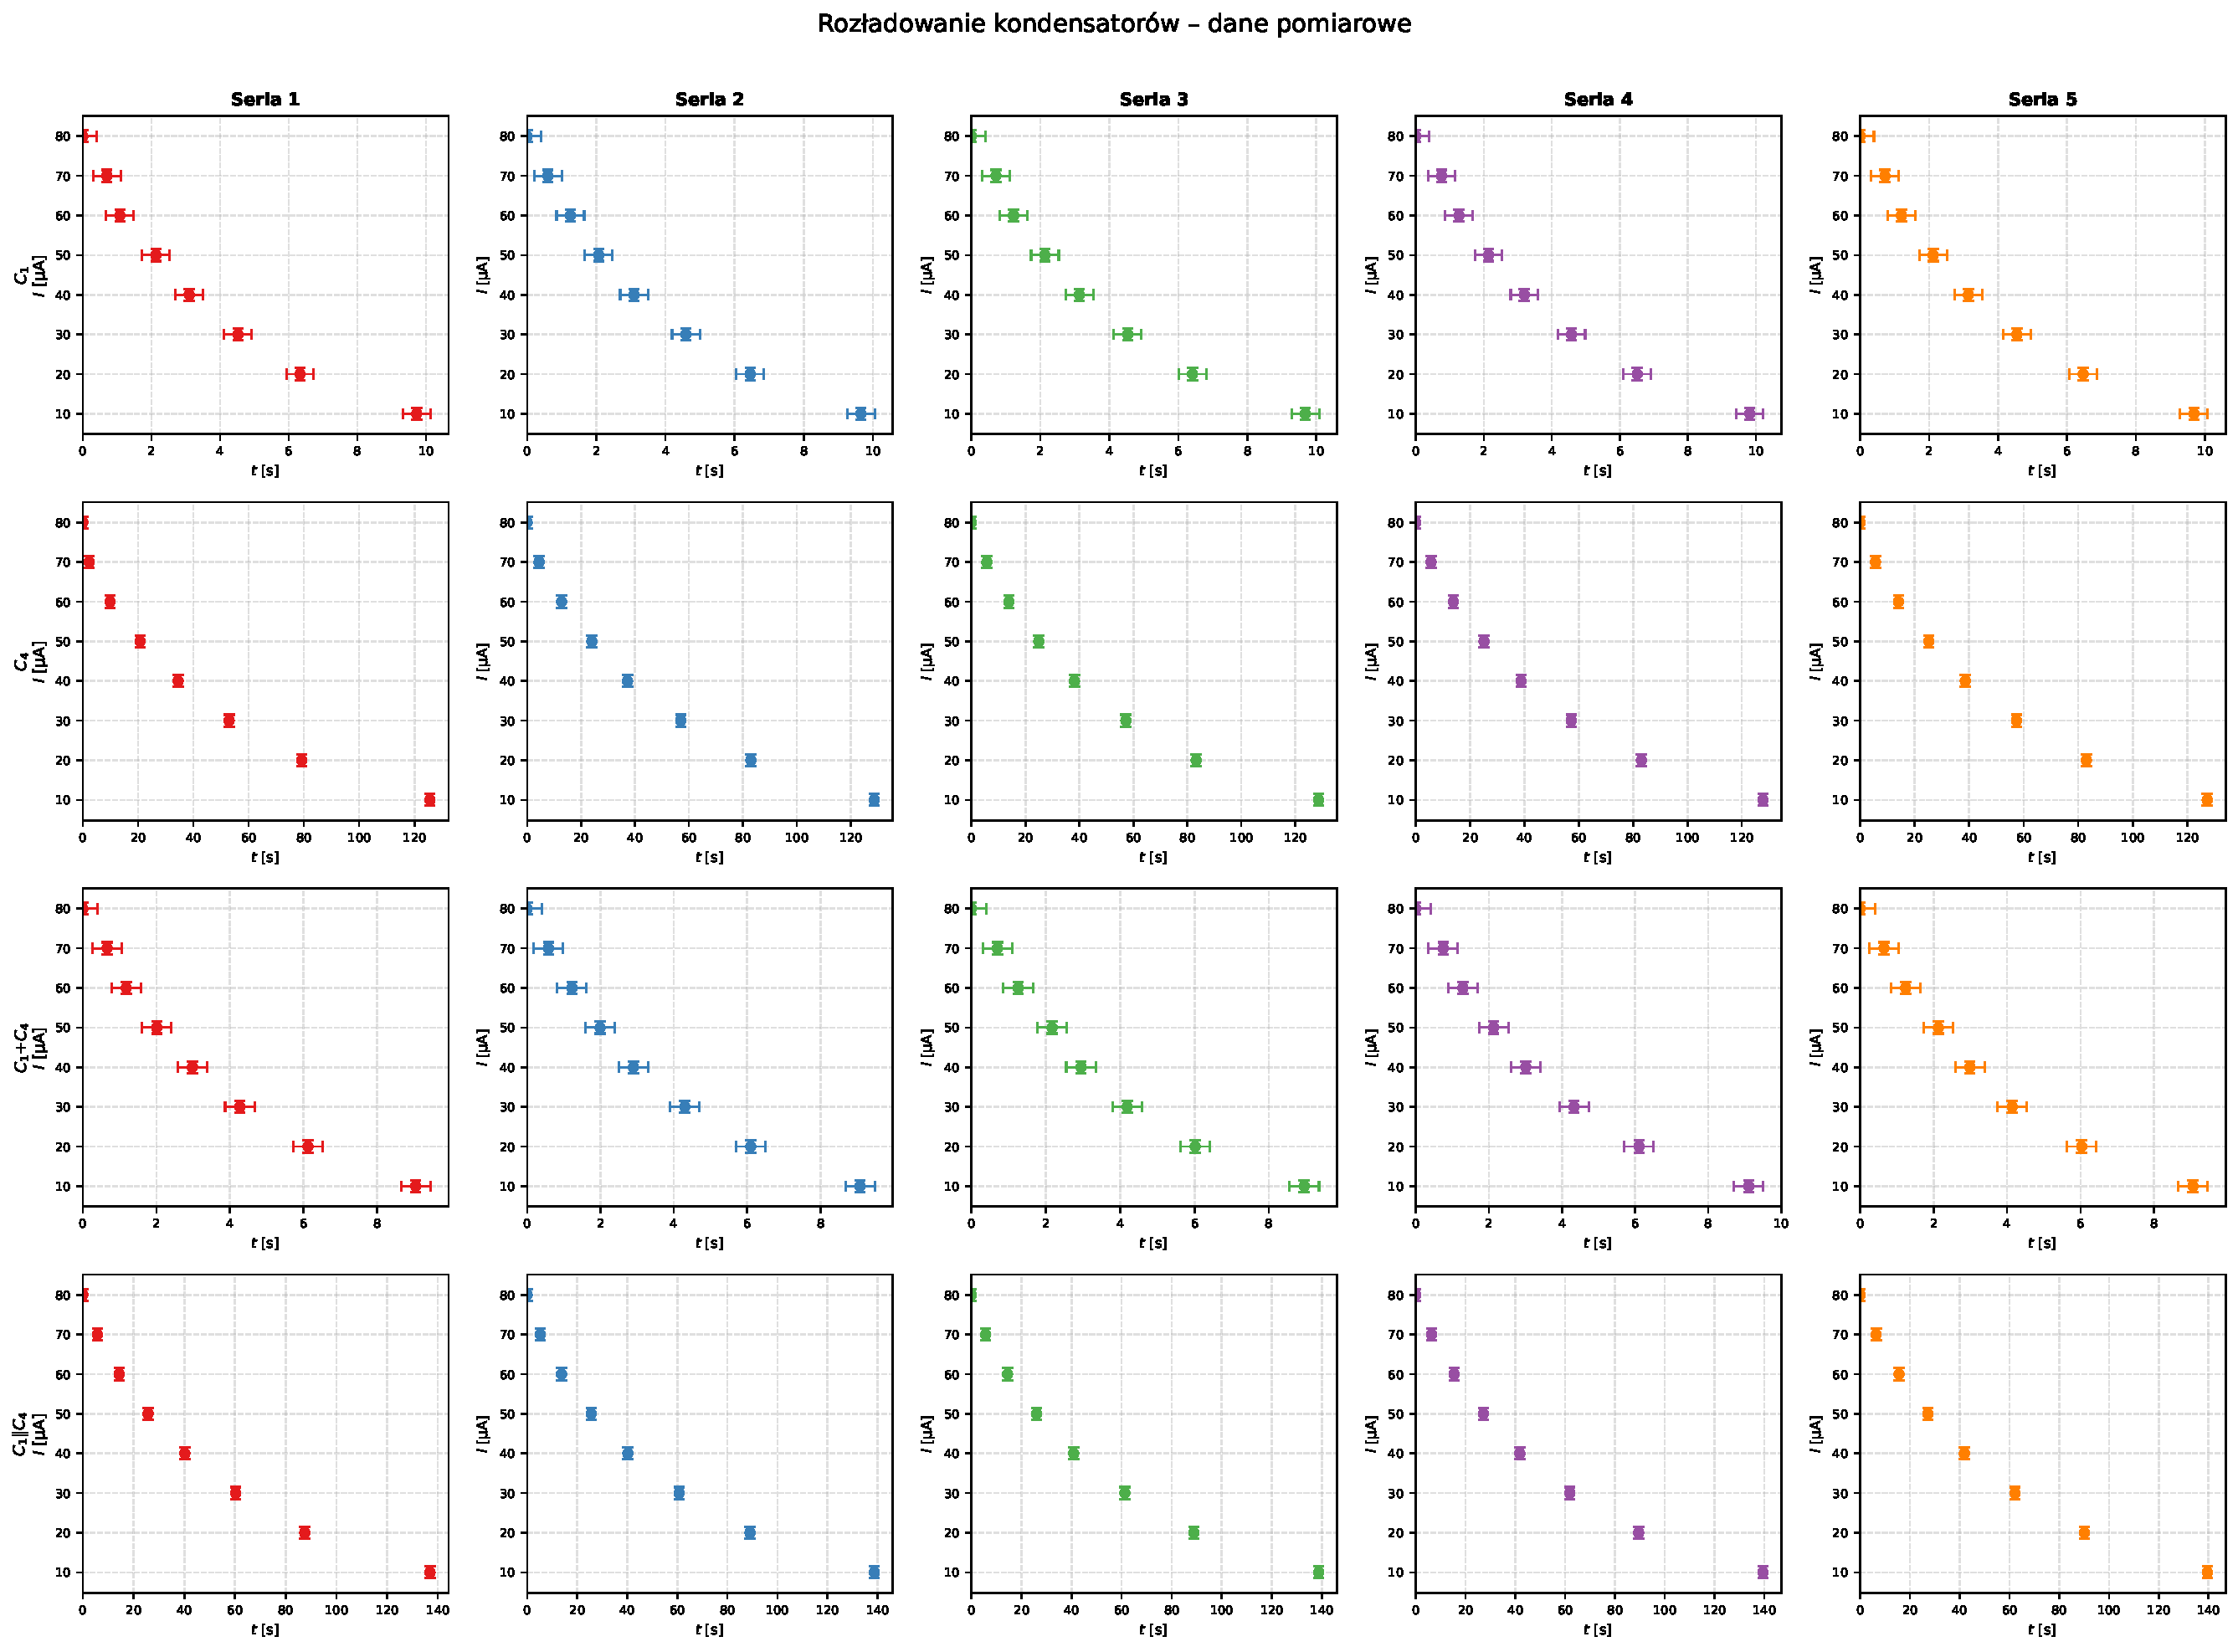
\includegraphics[width=\textwidth]{wykresy_punkty.pdf}
    \caption{Zależność natężenia prądu rozładowania $I$ od czasu $t$
             dla wszystkich badanych układów kondensatorów.
             Punkty --- dane pomiarowe z pięciu serii.
             Czasy przesunięte tak, aby $t = 0$ odpowiadało chwili,
             gdy $I = \SI{80}{\micro\ampere}$.}\label{fig:punkty}
\end{figure}

\begin{figure}[H]
    \centering
    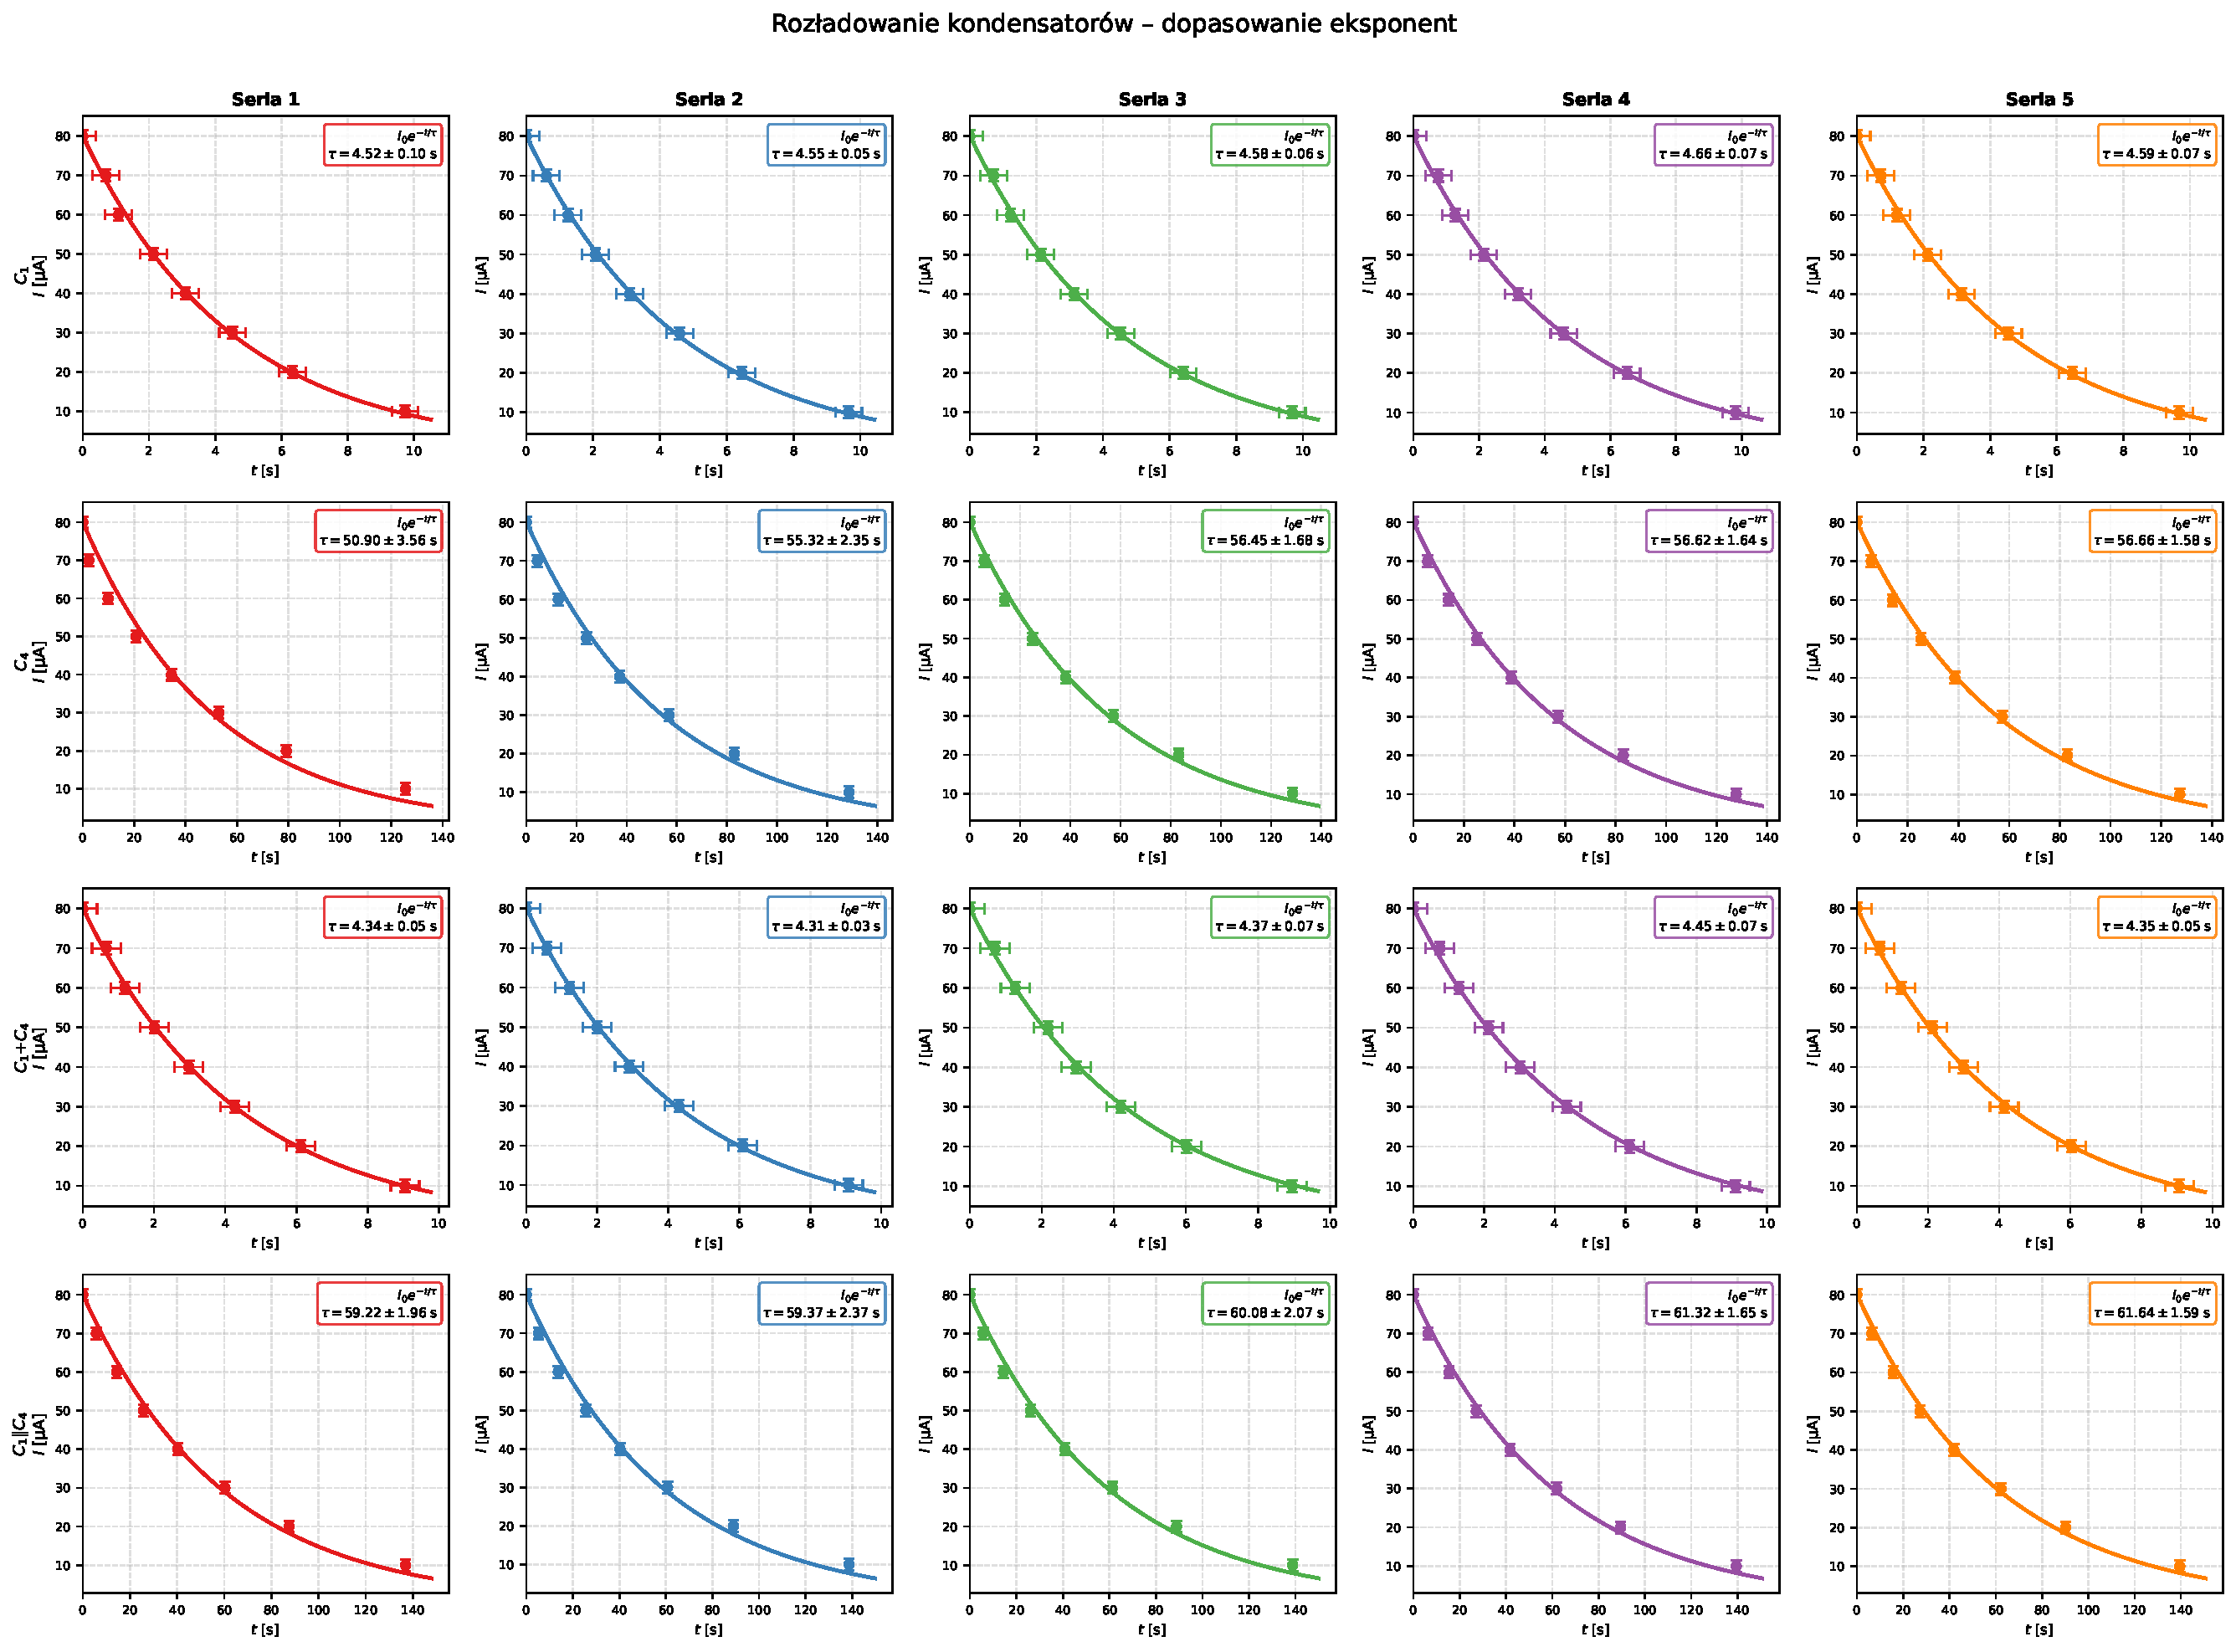
\includegraphics[width=\textwidth]{wykresy_eksponenty.pdf}
    \caption{Dopasowanie krzywej wykładniczej $I = I_0\,e^{-t/\tau}$ do danych
             pomiarowych (regresja nieliniowa). Czasy przesunięte jak
             na rys.~\ref{fig:punkty}.}\label{fig:eksponenty}
\end{figure}

\begin{figure}[H]
    \centering
    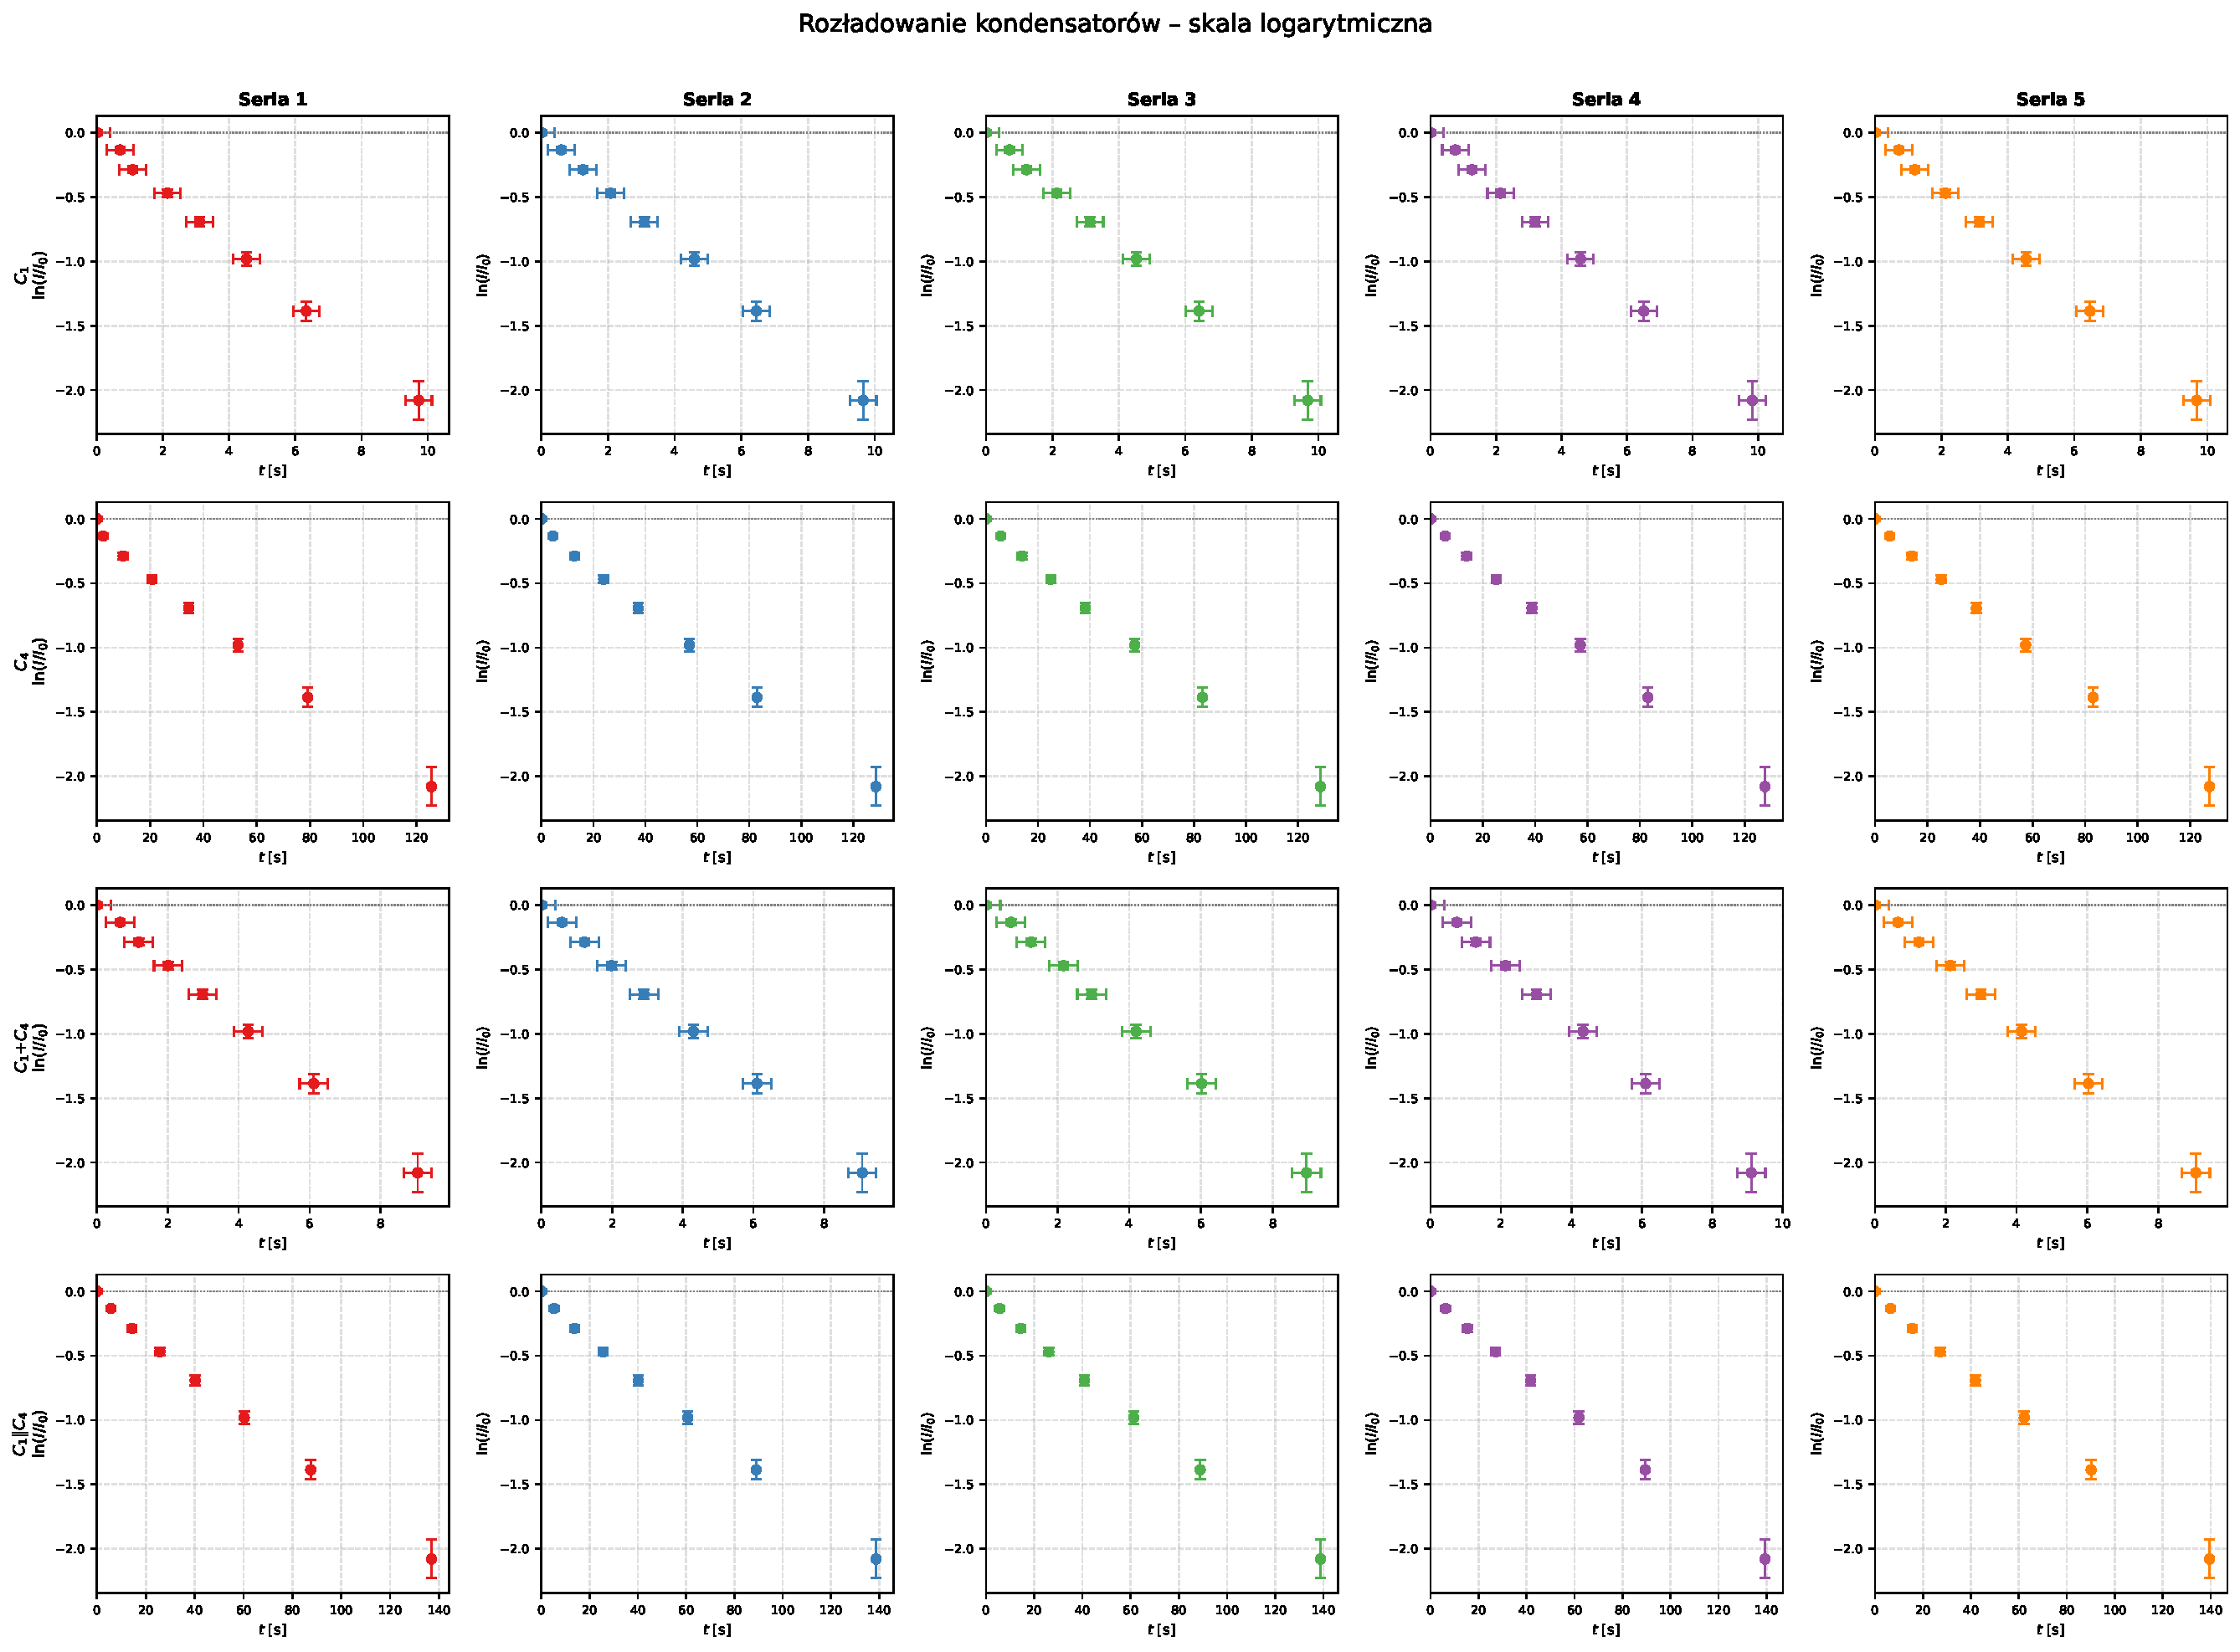
\includegraphics[width=\textwidth]{wykresy_log.pdf}
    \caption{Dane pomiarowe w skali logarytmicznej --- zależność $\ln(I/I_0)$ od
             czasu $t$. Czasy przesunięte jak na rys.~\ref{fig:punkty}.}\label{fig:log}
\end{figure}

\begin{figure}[H]
    \centering
    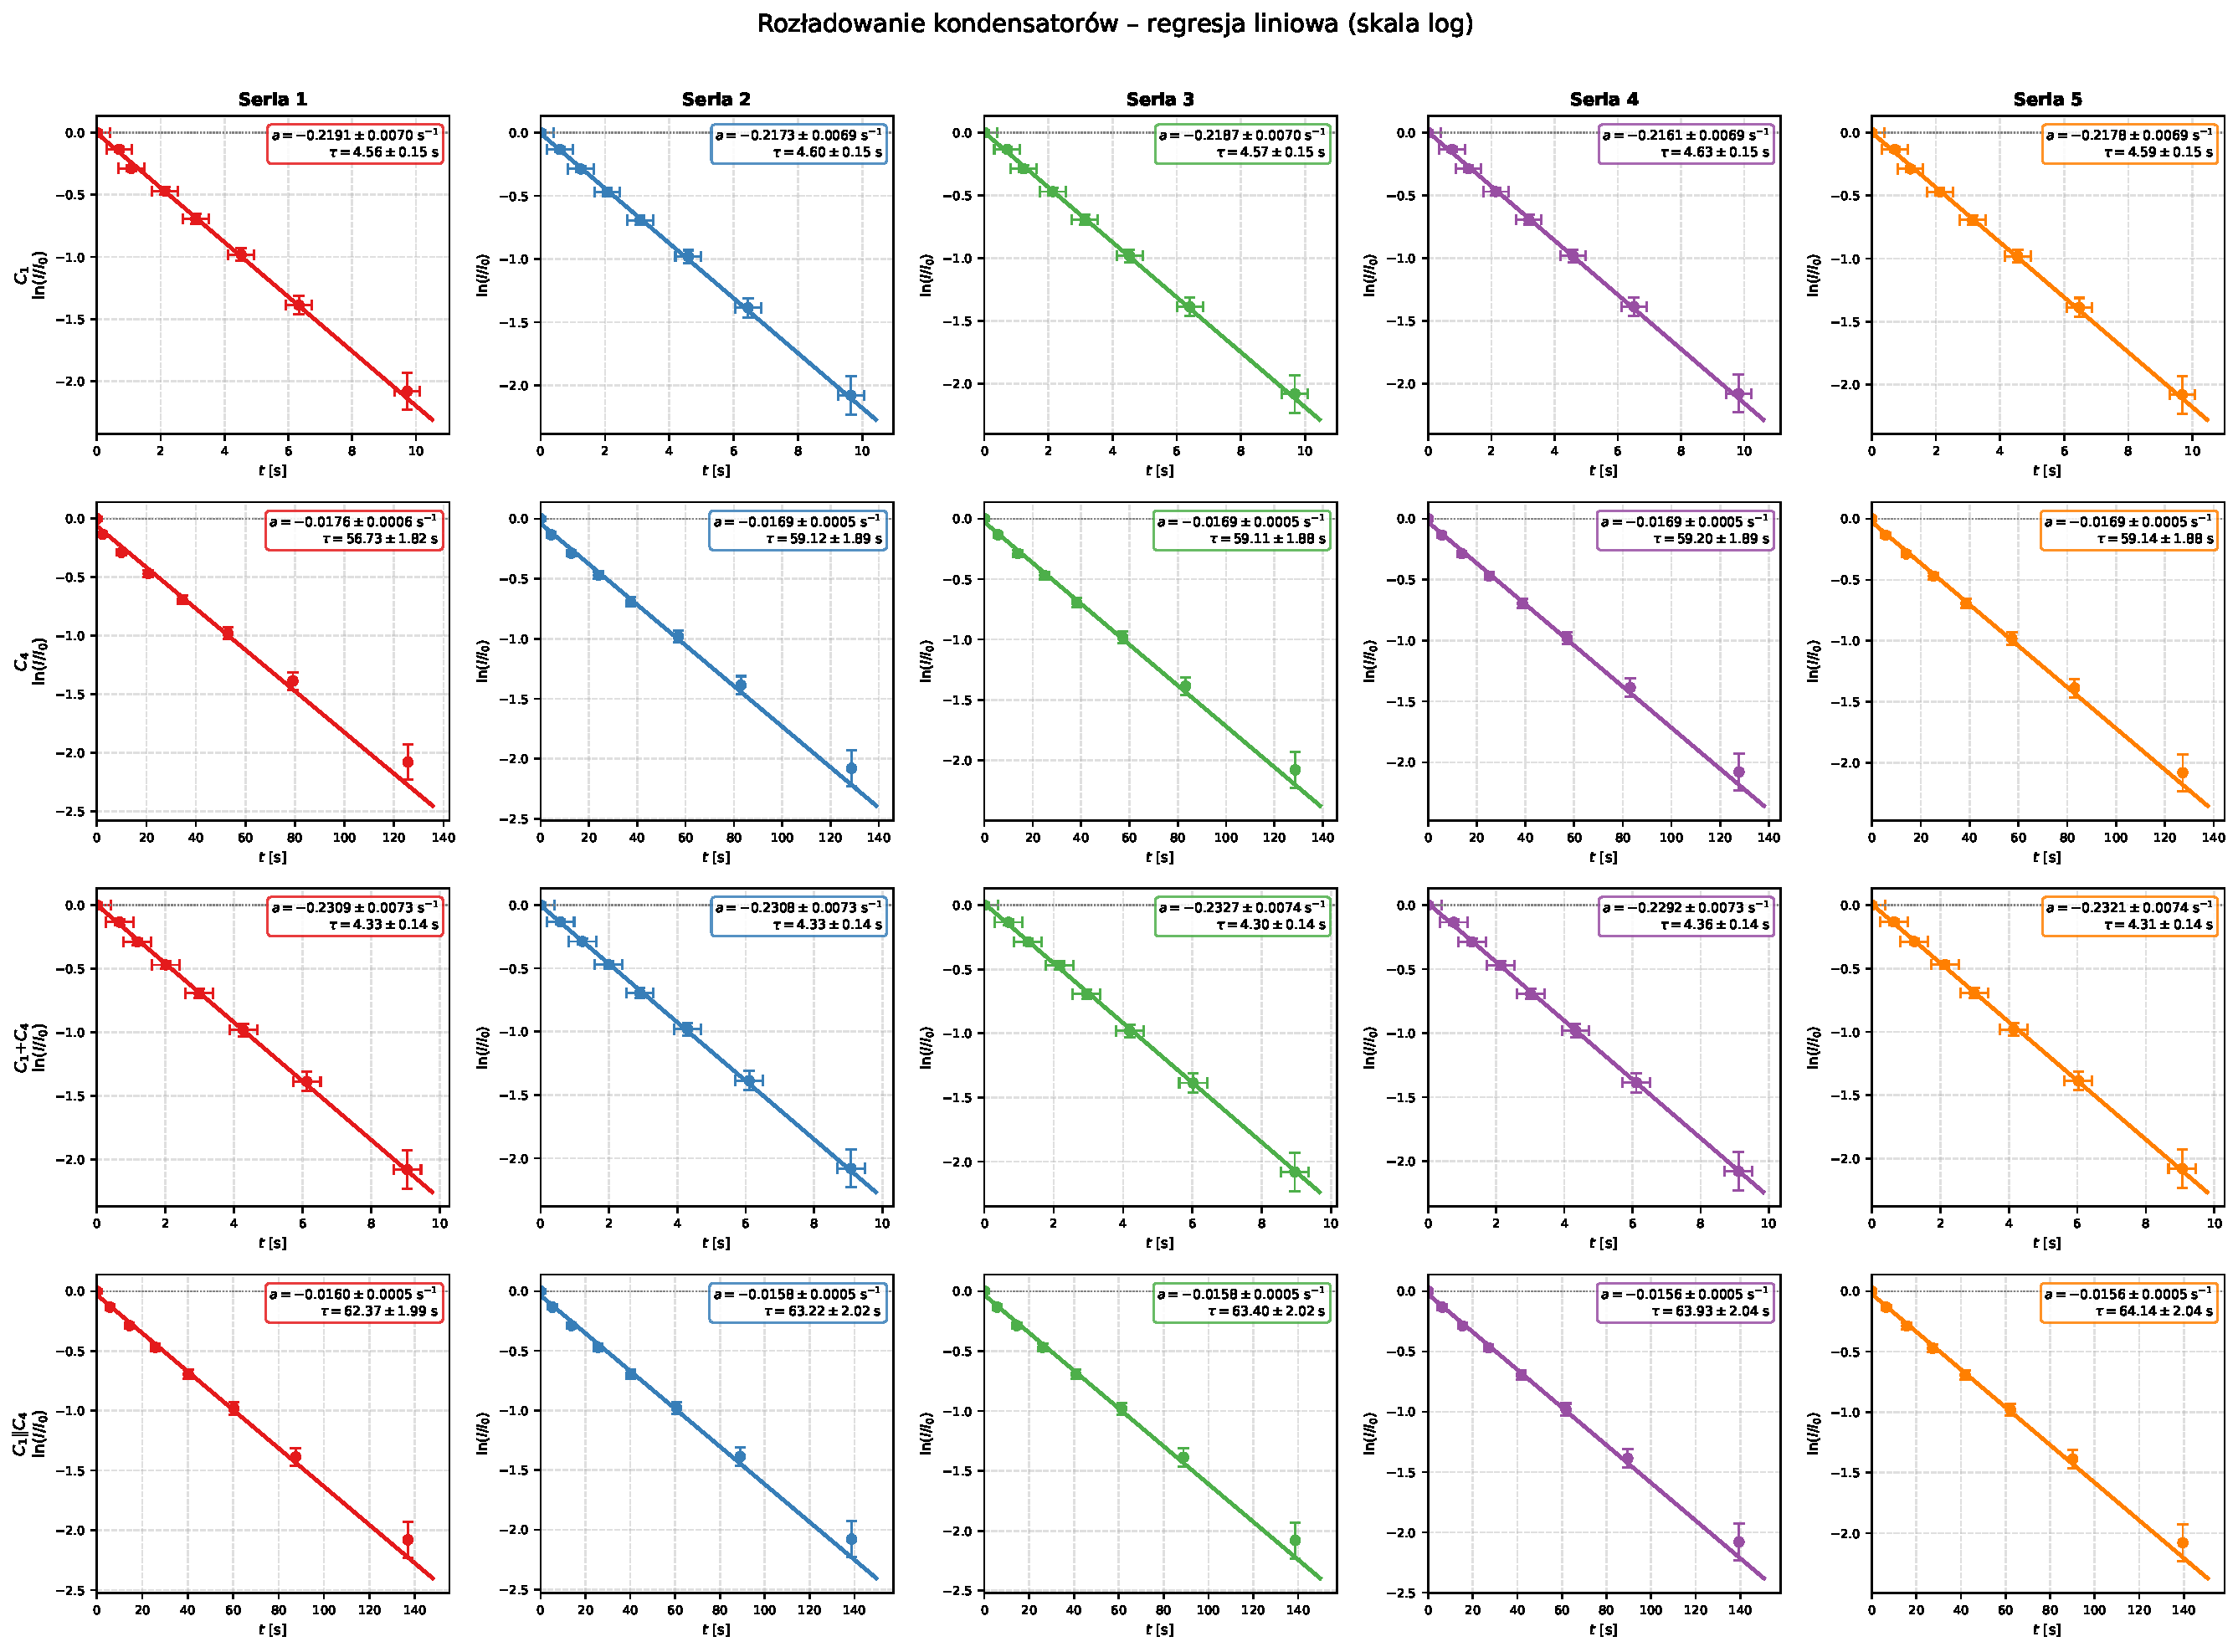
\includegraphics[width=\textwidth]{wykresy_log_regresja.pdf}
    \caption{Regresja liniowa $\ln(I/I_0) = at + b$ (nachylenie $a = -1/\tau$)
             w skali logarytmicznej. Czasy przesunięte jak
             na rys.~\ref{fig:punkty}.}\label{fig:log_regresja}
\end{figure}

% -------------------------------------------
\section{Opracowanie wyników}
% -------------------------------------------

Stałe czasowe $\tau$ wyznaczono dwoma niezależnymi metodami dla każdego układu
kondensatorów, a~następnie obliczono ważoną średnią z~pięciu serii pomiarowych.
Wyniki porównano w~tabeli~\ref{tab:tau}.

\paragraph{Metoda regresji liniowej.}
Z równania~(\ref{eq:log}) wynika, że zależność $\ln(I/I_0)$ od czasu~$t$ powinna
być liniowa z~nachyleniem $a = -1/\tau$. Do punktów każdej serii dopasowano prostą
$\ln(I/I_0) = at + b$ metodą ważonej regresji liniowej z~wagami
$w_i = 1/u_{\ln,i}^2$, gdzie $u_{\ln} = u_I/I$ (rys.~\ref{fig:log_regresja}).
Stałą czasową wyznaczono ze wzoru:
\begin{equation}
    \tau_\text{lin} = -\frac{1}{a}, \qquad
    u_{\tau_\text{lin}} = \frac{u_a}{a^2}.
    \label{eq:tau_lin}
\end{equation}
Niepewność $u_{I_0}$ nie wchodzi do $u_{\tau_\text{lin}}$: ponieważ $I_0$ jest
stałą odejmowaną od wszystkich $y_i = \ln(I_i/I_0)$, jej błąd powoduje
jednorodne przesunięcie wszystkich punktów o~$\delta = u_I/I_0$, co zmienia
tylko wyraz wolny~$b$, a~nie nachylenie~$a$.

\paragraph{Metoda dopasowania eksponenty.}
Stałą czasową wyznaczono również przez bezpośrednie dopasowanie funkcji
wykładniczej~(\ref{eq:eksponenta}) do danych $I(t)$ metodą nieważonej regresji
nieliniowej (rys.~\ref{fig:eksponenty}).

\begin{table}[H]
\centering
\caption{Stałe czasowe $\tau$ wyznaczone obiema metodami (ważona średnia z~5~serii).}\label{tab:tau}
\begin{tabular}{l r @{\;$\pm$\;} r r @{\;$\pm$\;} r}
\toprule
Układ & \multicolumn{2}{c}{$\tau_\text{lin}$ [s]} & \multicolumn{2}{c}{$\tau_\text{exp}$ [s]} \\
\midrule
$C_1$                   & $4{,}591$ & $0{,}065$ & $4{,}581$ & $0{,}028$ \\
$C_4$                   & $58{,}63$ & $0{,}84$  & $56{,}09$ & $0{,}85$  \\
$C_1$, $C_4$ szeregowo  & $4{,}327$ & $0{,}062$ & $4{,}343$ & $0{,}021$ \\
$C_1$, $C_4$ równolegle & $63{,}40$ & $0{,}90$  & $60{,}58$ & $0{,}84$  \\
\bottomrule
\end{tabular}
\end{table}

Dla kondensatora $C_1$ i~połączenia szeregowego obie metody dają wyniki zgodne
w~granicach niepewności. Dla $C_4$ i~połączenia równoległego stałe czasowe
z~regresji liniowej są systematycznie wyższe o~ok.\ 4\% od tych uzyskanych
z~dopasowania eksponenty. Przyczyną jest różnica modeli statystycznych.
Regresja liniowa stosuje wagi $w_i = {(I_i/u_I)}^2$, dzięki czemu punkty
o~dużym~$I$ (wczesny czas, mała niepewność względna $u_{\ln} = u_I/I$)
dominują w~dopasowaniu --- jest to właściwe uwzględnienie heteroskedastyczności
wynikającej z~transformacji logarytmicznej. Nieważona regresja nieliniowa
traktuje wszystkie punkty jednakowo; dla układów o~dużej stałej czasowej
pomiary przy małym~$I$ (duże~$t$, duża niepewność względna) mają nadmierny
wpływ i~``ciągną'' $\tau_\text{exp}$ ku mniejszym wartościom.
Dalsze obliczenia prowadzono na podstawie $\tau_\text{lin}$.

\subsection{Pojemności kondensatorów z regresji liniowej}

Pojemność każdego układu wyznaczono ze wzoru $C = \tau_\text{lin}/R$.
Niepewność obliczono metodą różniczki zupełnej:
\begin{equation}
    u_C = \sqrt{{\left(\frac{u_\tau}{R}\right)}^{\!2}
               + {\left(\frac{\tau\, u_R}{R^2}\right)}^{\!2}}.
    \label{eq:uC}
\end{equation}
Wyniki zestawiono w~tabeli~\ref{tab:cap_fit}.

\begin{table}[H]
\centering
\caption{Pojemności wyznaczone z~regresji liniowej ($C = \tau_\text{lin}/R$,\;
         $R = \SI{77700 \pm 50}{\ohm}$).}\label{tab:cap_fit}
\begin{tabular}{l r @{\;$\pm$\;} r}
\toprule
Układ & \multicolumn{2}{c}{$C$ [$\mu$F]} \\
\midrule
$C_1$                   & $59{,}09$ & $0{,}84$ \\
$C_4$                   & $755$     & $11$     \\
$C_1$, $C_4$ szeregowo  & $55{,}68$ & $0{,}79$ \\
$C_1$, $C_4$ równolegle & $816$     & $12$     \\
\bottomrule
\end{tabular}
\end{table}

\subsection{Pojemności zastępcze --- porównanie metod}

Pojemności zastępcze wyznaczono dwoma sposobami: z~regresji liniowej (tabela~\ref{tab:cap_fit})
oraz ze wzorów~(\ref{eq:rownoleg}) i~(\ref{eq:szereg}) na podstawie pojemności
pojedynczych kondensatorów. Niepewności obliczono różniczką zupełną:
\begin{align}
    u_{C_r} &= \sqrt{u_{C_1}^2 + u_{C_4}^2}, \label{eq:uCr}\\
    u_{C_s} &= C_s^2\sqrt{{\left(\frac{u_{C_1}}{C_1^2}\right)}^{\!2}
                          + {\left(\frac{u_{C_4}}{C_4^2}\right)}^{\!2}}. \label{eq:uCs}
\end{align}
Wyniki porównano w~tabeli~\ref{tab:cap_compare}.

\begin{table}[H]
\centering
\caption{Porównanie pojemności zastępczych wyznaczonych metodą fitowania
         i~ze wzorów.}\label{tab:cap_compare}
\begin{tabular}{l l r @{\;$\pm$\;} r}
\toprule
Połączenie & Metoda & \multicolumn{2}{c}{$C$ [$\mu$F]} \\
\midrule
\multirow{2}{*}{Równolegle}
  & fit           & $816$     & $12$     \\
  & wzór          & $814$     & $11$     \\
\addlinespace
\multirow{2}{*}{Szeregowo}
  & fit           & $55{,}68$ & $0{,}79$ \\
  & wzór          & $54{,}80$ & $0{,}73$ \\
\bottomrule
\end{tabular}
\end{table}

Obie metody dają wyniki zgodne w~granicach niepewności pomiarowych.

\subsection{Ładunki zgromadzone na kondensatorach}

Ładunek zgromadzony na okładkach kondensatora wyznaczono ze wzoru~(\ref{eq:ladunek_tau}):
$q = \tau_\text{lin} I_0$, gdzie $I_0 = \SI{80}{\micro\ampere}$.
Niepewność obliczono różniczką zupełną z uwzględnieniem niepewności obu wielkości:
\begin{equation}
    u_q = \sqrt{{\left(I_0\, u_{\tau}\right)}^{\!2}
               + {\left(\tau\, u_I\right)}^{\!2}}.
    \label{eq:uq}
\end{equation}

\begin{table}[H]
\centering
\caption{Ładunki zgromadzone na kondensatorach ($I_0 = \SI{80}{\micro\ampere}$,
         $u_I = \SI{1,5}{\micro\ampere}$).}\label{tab:charge}
\begin{tabular}{l r @{\;$\pm$\;} r}
\toprule
Układ & \multicolumn{2}{c}{$q$ [$\mu$C]} \\
\midrule
$C_1$                   & $367{,}3$ & $8{,}6$  \\
$C_4$                   & $4690$    & $110$    \\
$C_1$, $C_4$ szeregowo  & $346{,}2$ & $8{,}2$  \\
$C_1$, $C_4$ równolegle & $5070$    & $120$    \\
\bottomrule
\end{tabular}
\end{table}

% -------------------------------------------
\section{Wnioski}
% -------------------------------------------

Metodą rozładowania kondensatora w~obwodzie RC wyznaczono pojemności dwóch
kondensatorów:
\[
    C_1 = (59{,}09 \pm 0{,}84)\;\mu\mathrm{F}, \qquad
    C_4 = (755 \pm 11)\;\mu\mathrm{F}.
\]
Pojemności kondensatorów różnią się ponad dwunastokrotnie; oba wyniki obarczone
są niepewnością względną poniżej~1{,}5\%.

Sprawdzono wzory na pojemność zastępczą baterii kondensatorów. Przy połączeniu
równoległym uzyskano $C_r^\text{(fit)} = (816 \pm 12)\;\mu\mathrm{F}$
oraz $C_r^\text{(wzór)} = C_1 + C_4 = (814 \pm 11)\;\mu\mathrm{F}$;
wyniki są zgodne w~granicach niepewności, co potwierdza wzór~(\ref{eq:rownoleg}).
Przy połączeniu szeregowym $C_s^\text{(fit)} = (55{,}68 \pm 0{,}79)\;\mu\mathrm{F}$
i~$C_s^\text{(wzór)} = (54{,}80 \pm 0{,}73)\;\mu\mathrm{F}$ --- również zgodne,
co potwierdza wzór~(\ref{eq:szereg}).

Porównanie dwóch metod wyznaczania stałej czasowej wykazało, że dla układów
o~małej stałej czasowej ($C_1$, $C_1{+}C_4$ szeregowo, $\tau \approx 4{,}3$--$4{,}6\;\mathrm{s}$)
obie metody dają zgodne wyniki. Dla układów o~dużej stałej czasowej ($C_4$,
$C_1\|C_4$ równolegle, $\tau \approx 58$--$63\;\mathrm{s}$) regresja liniowa
zwraca wartości o~ok.~4\% wyższe niż dopasowanie eksponenty. Przyczyną jest
różnica w~sposobie ważenia punktów: regresja liniowa właściwie uwzględnia
heteroskedastyczność wynikającą z~transformacji logarytmicznej (wagi
$w_i = {(I_i/u_I)}^2$ faworyzują punkty o~małej niepewności względnej),
podczas gdy nieważona regresja nieliniowa traktuje wszystkie punkty jednakowo
i~nadmiernie eksponuje pomiary przy małym~$I$, które mają dużą niepewność
względną. Dla układów o~dużej stałej czasowej te punkty stanowią znaczną
część zakresu pomiarowego, co tłumaczy obserwowaną rozbieżność.

Głównymi źródłami niepewności były: czas reakcji operatora ($u_t = 0{,}4\;\mathrm{s}$)
oraz rozdzielczość mikroamperomierza ($u_I = 1{,}5\;\mu\mathrm{A}$).

\begin{thebibliography}{9}
\bibitem{skrypt}
\textit{Skrypt do ćwiczeń laboratoryjnych z fizyki, I Pracownia Fizyczna}, ćwiczenie E11.
\end{thebibliography}

\end{document}
% =============================================
